\documentclass[conference]{IEEEtran}
\IEEEoverridecommandlockouts
% The preceding line is only needed to identify funding in the first footnote. If that is unneeded, please comment it out.
\usepackage{cite}
\usepackage{amsmath,amssymb,amsfonts}
\usepackage{algorithm}
\usepackage{algpseudocode}
\usepackage{graphicx}
\usepackage{textcomp}
\usepackage{xcolor}
\usepackage{multirow}
\usepackage{subfig}
\usepackage{url}
\usepackage{booktabs}
\usepackage{bm}
\usepackage{array}
\usepackage{tikz,pgfplots}
\newcommand{\rr}{\color{red}}
\newcommand{\ourwork}{OurWork}
\def\BibTeX{{\rm B\kern-.05em{\sc i\kern-.025em b}\kern-.08em
    T\kern-.1667em\lower.7ex\hbox{E}\kern-.125emX}}
\begin{document}

\title{
% Unifying Long-Context Inference on NPUs with a Causal Operator for Separable Matrices
Context-Driven Performance Modeling for Causal Inference Operators on Neural Processing Units
}


\author{
\IEEEauthorblockN{Neelesh Gupta, Rakshith Jayanth, Dhruv Parikh, Viktor Prasanna}
\IEEEauthorblockA{
   University of Southern California, Los Angeles, California, USA \\
    neeleshg@usc.edu, jayanthr@usc.edu, dhruvash@usc.edu, prasanna@usc.edu}
}


\maketitle
\begin{abstract}
The proliferation of large language models (LLMs) has driven demand for long-context inference on resource-constrained edge devices. However, deploying these models on Neural Processing Units (NPUs) presents significant challenges due to the architectural mismatch: quadratic complexity of standard attention mechanisms conflicts with memory and compute patterns of edge accelerators. This paper presents a comprehensive performance analysis of various causal inference operators on a modern NPU. We benchmark standard quadratic attention against several sub-quadratic alternatives, including structured state-space and linear attention models. Our analysis reveals that while sub-quadratic methods offer superior scalability, they introduce distinct computational bottlenecks on the NPU's specialized execution units. We identify that quadratic attention becomes severely memory-bound, suffering from cache inefficiency and pipeline stalls exceeding 95\% at long contexts. In contrast, sub-quadratic models can become compute-bound on programmable vector cores. These findings provide critical insights for the co-design of hardware-aware models and optimization strategies to enable on-device AI inference with long-contexts.
\end{abstract}

\begin{IEEEkeywords}
Long-context inference, NPU, causal attention
\end{IEEEkeywords}
\section{Introduction}

Long-context inference has become essential for document understanding, conversational AI, and real-time decision systems~\cite{chung2025long, qian2024long}. Applications from medical record analysis to legal contract review increasingly demand processing of 100K+ token sequences. While cloud solutions can handle these workloads, privacy concerns, latency requirements, and operational costs are driving deployment to edge devices. Modern edge platforms now integrate Neural Processing Units (NPUs)—specialized accelerators that deliver exceptional efficiency for data-parallel operations but face severe constraints: limited scratchpad memory (typically 2-4MB), systolic execution patterns, and strict power budgets.

Transformer-based models like Llama deliver state-of-the-art quality but require quadratic computation and linear memory growth with context length~\cite{dao2022flash}. At just 16K tokens, the Key-Value cache consumes over 768MB—more than 30x the capacity of leading NPUs. State-space models (SSMs) like Mamba offer linear scaling but underutilize NPU parallelism due to their recurrent nature during autoregressive decoding inference~\cite{gu2024mamba}. This fragmentation forces practitioners into hardware-specific compromises, limiting adoption of long-context capabilities where they're needed most: on-device.

Recent works have looked into hybrid architectures or ways towards creating a general class of operators for causal inference~\cite{dao2024ssd, lieber2024jambahybridtransformermambalanguage, dong2024hymbahybridheadarchitecturesmall}. While these efforts advance the theoretical understanding, a critical gap remains in characterizing how these diverse operators perform on real-world, resource-constrained hardware like NPUs. The architectural trade-offs made by these models—such as prioritizing data locality, computational regularity, or state compression—have profound, yet unquantified, implications for on-device performance. This paper bridges that gap by providing a comprehensive performance analysis and modeling of causal inference operators on a modern NPU. We move beyond theoretical complexity and provide a rigorous empirical study of latency, throughput, and hardware utilization, culminating in a Roofline analysis that explains the performance landscape.

\subsection{Our Contributions}
This work provides a detailed characterization of attention mechanisms on edge NPUs. Our key contributions are:
\begin{itemize}
    \item A comprehensive performance benchmark of quadratic and sub-quadratic attention operators on a real-world NPU, analyzing latency, throughput, and pipeline efficiency.
    \item Identification and analysis of critical performance bottlenecks, demonstrating that quadratic attention becomes memory-bound due to cache inefficiency while sub-quadratic models become compute-bound on specialized vector units.
    \item A quantitative Roofline performance model that explains the performance limitations of each operator class in terms of the NPU's architectural constraints.
    \item Actionable insights for co-designing hardware-aware models and compiler optimizations to enable efficient long-context inference on the edge.
\end{itemize}
% \section{Introduction}

% Long-context inference has become essential for document understanding, conversational AI, and real-time decision systems~\cite{chung2025long, qian2024long}. Applications from medical record analysis to legal contract review increasingly demand processing of 100K+ token sequences. While cloud solutions can handle these workloads, privacy concerns, latency requirements, and operational costs are driving deployment to edge devices. Modern edge platforms now integrate Neural Processing Units (NPUs)—specialized accelerators that deliver exceptional efficiency for data-parallel operations but face severe constraints: limited scratchpad memory (typically 24MB), systolic execution patterns, and strict power budgets.

% Transformer-based models like Llama deliver state-of-the-art quality but require quadratic computation and linear memory growth with context length~\cite{dao2022flash}. At just 16K tokens, the Key-Value cache consumes over 768MB—32× the capacity of leading NPUs. State-space models (SSMs) like Mamba offer linear scaling but underutilize NPU parallelism due to their recurrent nature during autoregressive decoding inference~\cite{gu2024mamba}. This fragmentation forces practitioners into hardware-specific compromises, limiting adoption of long-context capabilities where they're needed most: on-device.

% Recent works have looked into hybrid architectures and working towards creating general class of operators for causal inference~\cite{dao2024ssd}.
% We introduce \ourwork, a unified approach to long-context inference that transcends the attention-SSM dichotomy. Our core insight is that both model families share an underlying mathematical structure—semi-separable computation—that can be optimized for NPU constraints. By dynamically adapting execution strategies to hardware resources, \ourwork enables transformer-quality inference at SSM efficiencies, scaling linearly to 128K+ contexts on edge devices.

% Our contributions can be summarized as follows:
% \begin{itemize}
% \item We unify attention and state-space models under a single computational framework by exploiting their shared semi-separable structure, eliminating hardware fragmentation.
% \item We develop a hardware-aware operator that dynamically switches execution modes—\textit{parallel} (Toeplitz-structured) for short sequences, \textit{sequential} (recurrent) for moderate contexts, and \textit{chunked} (hierarchical) for extreme lengths—based on NPU constraints.
% \item We introduce three NPU-specific innovations: 
%   \begin{enumerate}
%     \item Register-blocked chunking for maximal scratchpad utilization
%     \item Fixed state compression via efficient summarization
%     \item Toeplitz-structured attention kernels optimized for systolic arrays
%   \end{enumerate}
% \item We demonstrate linear-scaling inference to 128K contexts on Intel Core Ultra NPUs, achieving 4.2$\times$ speedup over SSMs while maintaining transformer-level accuracy.
% \end{itemize}






\section{Background}
\label{sec:background}

\subsection{Fundamental Tradeoff for Long-Context Inference}
Autoregressive sequence modeling faces dual constraints: \textit{memory complexity} for context retention and \textit{computational complexity} for state evolution. For sequence length $N$ and model dimension $D$, we observe:

\begin{equation}
\underbrace{\text{Memory}}_{\text{Context}} \sim O(N \cdot D), \quad 
\underbrace{\text{Compute}}_{\text{Inference}} \sim O(N^2 \cdot D)
\end{equation}

\noindent\textbf{Prefill Phase:} Computes initial context representation:
\begin{equation}
\mathcal{C} = f_{\theta}(X_{1:N}) \quad 
\begin{cases} 
\text{Attention: } \mathcal{C} = \{K,V\}_{1:N} \\
\text{SSM: } \mathcal{C} = h_N
\end{cases}
\end{equation}

\noindent\textbf{Decode Phase:} Updates state incrementally:
\begin{equation}
y_t, \mathcal{C}_t = g_{\theta}(x_t, \mathcal{C}_{t-1})
\end{equation}

\noindent\textbf{Memory-State Tradeoff.}
Architectures balance expressiveness against hardware constraints as we show in Figure \ref{fig:tradeoff}:
\begin{itemize}
    \item \textit{Attention-based models} (Llama): Maintain explicit KV cache ($O(N \cdot D)$ memory) enabling rich context access.
    \item \textit{State-space models} (Mamba): Compress context to fixed-size state $h_t$ ($O(D)$ memory) at additional computational cost.
\end{itemize}

We introduce this tradeoff not only to compare model classes, but also because it forms the architectural basis for the structured operators analyzed in this paper. Many recent causal inference variants—such as Toeplitz, Retentive, and Fourier—draw inspiration from state-space models, embedding recurrent or convolutional priors directly into attention layers~\cite{sun2023retentivenetworksuccessortransformer, gu2024mamba, dao2024ssd, poli2023hyena, peng2023rwkv}. These hybrid mechanisms blend the long-range capacity of traditional attention with the computational efficiency and inductive structure of SSMs, making the memory-state tradeoff a key element for evaluating modern causal operators on resource-constrained hardware platforms such as NPU.


\begin{figure}[h!]
    \centering
    \includegraphics[width=0.8\linewidth]{fig/my_tradeoff.pdf}
    \caption{Differences in persistent memory and layer-wise dataflow for Attention-based Llama vs. SSM-based Mamba.}
    \label{fig:tradeoff}
\end{figure}

\subsection{Heterogeneous Edge Platform with Neural Processing Units (NPU)}
State-of-the-art heterogeneous edge platforms—such as Intel Core Ultra processors (Intel AI PC)—combine traditional multi-core CPUs with specialized accelerators, including Graphics Processing Units (GPUs) and Neural Processing Units (NPUs). These diverse compute elements are integrated into a single System-on-Chip (SoC) architecture, featuring a unified system memory that facilitates seamless communication and efficient data sharing across all cores.


\begin{figure}[h]
\centering
\includegraphics[width=0.5\textwidth]{fig/npu.pdf}
\caption{NPU dataflow architecture with processing elements (PEs) and accumulator hierarchy. Note the absence of high-bandwidth memory for persistent state storage.}
\label{fig:npu-arch}
\end{figure}

Each of the three compute cores is designed to exploit specific types of workloads, leveraging their distinct system architectures and local memory hierarchies. The classic multi-core CPU, equipped with a three-level cache hierarchy, excels at handling general-purpose, logic-intensive workloads. GPUs feature Xe cores, each comprising multiple vector engines that are optimized for high data parallelism. Every Xe core includes a Shared Local Memory (SLM) block, accessible by all its vector engines to facilitate efficient intra-core communication.
In NPUs, compute acceleration is driven by the Data Path Unit (DPU), comprising of a PE array which employs a structured systolic array architecture to perform operations such as matrix multiplication with minimal data movement. NPUs also incorporate Streaming Hybrid Architecture Vector Engines (SHAVE), which support parallel execution of general-purpose tasks and activation function engine to efficiently compute activations. To further enhance efficiency, Direct Memory Access (DMA) engines are integrated into the NPU, enabling high-throughput data transfers from the global shared system memory to the local, software-managed cache. Due to their controlled data movement and predictable, statically scheduled execution flow, NPUs achieve higher energy efficiency for AI workloads compared to GPUs, which involve complex, dynamic execution patterns and data transfers. This energy efficiency is a critical requirement in resource-constrained edge computing environments, where power limitation is a significant design consideration.

\subsection{Causal Operators for Attention}

% \subsubsection{Attention-based Structured Masks}

\begin{figure}
    \centering
    \includegraphics[width=\linewidth]{fig/causal_matrices.pdf}
    \caption{From left to right, top to bottom are Full Causal, Toeplitz, Fourier, Retentive Decay, Semiseparable, and Linear Structured attention masks.}
    \label{fig:matrices}
\end{figure}

We describe in further detail which Causal Attention Masks we select to comprehensively survey and perform performance model analysis of a more general class of causal matrices seen in Figure \ref{fig:matrices}.

\noindent\textbf{Full Causal Mask:} The standard causal attention mechanism prevents tokens from attending to future positions using a triangular mask:
\[
\text{Attention}(Q,K,V) = \text{softmax}\left(\frac{QK^T}{\sqrt{d_k}} + M\right)V
\]
where $M$ is defined as:
\[
M_{ij} = \begin{cases} 
0 & i \geq j \\
-\infty & \text{otherwise}
\end{cases}
\]
This ensures position $i$ only attends to positions $j \leq i$.

\noindent\textbf{Linear Attention:} Replaces the softmax with kernel functions to enable linear complexity:
\[
\text{LinearAttention}(Q,K,V) = \phi(Q) (\phi(K))^T V
\]
where $\phi$ is a kernel function (in our implementation, low-rank projections). This reduces complexity from $O(N^2)$ to $O(N)$.

\noindent\textbf{Toeplitz Structured Attention~\cite{qin2023toeplitzneuralnetworksequence}:} Constrains the attention matrix to have constant diagonals:
\[
W_{ij} = \gamma^{|i-j|}
\]
\[
\text{ToeplitzAttention} = \text{softmax}(QK^T \odot W)V
\]
where $\gamma$ is a decay factor. This models position-based decay patterns.

\noindent\textbf{Fourier Structured Attention~\cite{tran2024fouriermixedwindowattentionaccelerating}:} Leverages the convolution theorem to compute attention in frequency domain:
\begin{align*}
Q_\omega &= \mathcal{F}(Q) \\
K_\omega &= \mathcal{F}(K) \\
V_\omega &= \mathcal{F}(V) \\
\text{FourierAttention} &= \mathcal{F}^{-1}(Q_\omega \odot \overline{K_\omega} \odot V_\omega)
\end{align*}
where $\mathcal{F}$ and $\mathcal{F}^{-1}$ are Discrete Fourier Transform (DFT) and Inverse DFT (IDFT) operations, respectively. This enables a computation complexity of $O(N \log N)$.

\noindent\textbf{Retentive Attention~\cite{sun2023retentivenetworksuccessortransformer}:} Introduces a decay mechanism that assigns exponentially decreasing weights to tokens based on relative position:
\[
W_{ij} = \begin{cases} 
\gamma^{i-j} & i \geq j \\
0 & \text{otherwise}
\end{cases}
\]
\[
\text{RetentiveAttention}(Q,K,V) = \text{softmax}\left(\frac{QK^T}{\sqrt{d_k}} \odot W\right)V
\]
where $\gamma \in (0,1)$ is the decay rate. This maintains causality while modeling recency bias in attention weights. Retentive attention provides tunable context compression and exhibits hardware-friendly diagonal structure.

% \subsubsection{State-Space Model-based Recurrence}

% State-space models with fixed-sized persistent state memory take on different compute graph models whether doing sequential inference or training, routing recurrent or convolution views of applying a state evolution matrix ($A$) on a hidden state $h_t$.

% \noindent\textbf{Recurrent Mode:} Computes the state sequence sequentially:
% \[
% h_t = Ah_{t-1} + Bx_t
% \]
% \[
% y_t = Ch_t
% \]
% where $A \in \mathbb{R}^{d_s \times d_s}$, $B \in \mathbb{R}^{d_s \times d_m}$, $C \in \mathbb{R}^{d_m \times d_s}$. This has $O(n)$ time complexity but sequential dependencies.

% \noindent\textbf{Parallel (Scan) Mode:} Computes the state sequence in parallel using prefix sums:
% \[
% h_t = \sum_{k=0}^t A^{t-k}Bx_k
% \]
% \[
% y = \text{cumsum}(X \ast B) \times A \times C
% \]
% where $\ast$ denotes matrix multiplication. This leverages parallel prefix algorithms for $O(\log n)$ depth.

\section{Microbenchmarking Kernels}

\subsection{Experimental Setup}
We conduct a series of microbenchmarks to evaluate the performance of various attention mechanisms on a Neural Processing Unit (NPU). The objective is to analyze device utilization and latency as a function of context length. All experiments are executed on a system with the hardware specifications detailed in Table \ref{tab:hardware_specs}. The NPU integrates a Digital Signal Processor (DSP) for control flow, a Data Path Unit (DPU) with a systolic array for matrix multiplication, programmable SIMD vector processors (SHAVE cores), and a high-bandwidth Direct Memory Access (DMA) engine.



\begin{table}[h]
\centering
\caption{Hardware Specifications}
\label{tab:hardware_specs}
\resizebox{\columnwidth}{!}{%
\begin{tabular}{@{}lcl@{}}
\toprule
\textbf{Component} & \textbf{Specification} & \textbf{Relevance} \\
\midrule
CPU & 16 cores (8P + 8E) & Control Logic \\
NPU & 10 TOPS @ 35W & Systolic Array Acceleration \\
DPU (PE Array) & 128$\times$128 INT8 & Matrix Multiplication \\
Scratchpad & 4 MB & Persistent State Storage \\
DMA Bandwidth & 64 GB/s & Data Movement \\
SHAVE Cores & 8 @ 1.4 GHz & Element-Wise Operations \\
Memory & 32 GB LPDDR5X & Global Buffer \\
\bottomrule
\end{tabular}%
}
\end{table}


\subsection{Device Utilization Analysis}
To understand the performance bottlenecks, we profile the execution time spent on the NPU's primary components: the DPU, DMA, and SHAVE cores. Table \ref{tab:utilization} presents the utilization breakdown for Fourier State-Space Attention (FSA) and Decayed Recurrent Attention (DRA), which serves as a proxy for retentive decay mechanisms.

For FSA, the workload is initially DPU-bound at shorter context lengths. However, as the context grows beyond 512 tokens, data movement becomes the dominant factor, and the model becomes \emph{DMA-bound}. This is primarily due to the $\operatorname{concat}$ operations required to manage the state, which saturate the DMA engine's bandwidth.

In contrast, DRA exhibits a different bottleneck. While initially compute-bound on the DPU, at context lengths of 1024 and greater, the workload transitions to being \emph{SHAVE-bound}. The $\operatorname{softmax}$ and element-wise multiply operations, which are offloaded to the programmable SHAVE cores, become the most time-consuming parts of the computation at long contexts.

\begin{table}[h]
\centering
\caption{Device Utilization Breakdown (\%). At long contexts, FSA becomes \emph{DMA-bound} while DRA becomes \emph{SHAVE-bound}.}
\label{tab:utilization}
\resizebox{\columnwidth}{!}{%
\begin{tabular}{@{}llccccl@{}}
\toprule
\textbf{Model} & \textbf{Context} & \textbf{DPU (\%)} & \textbf{DMA (\%)} & \textbf{SHAVE (\%)} & \textbf{Bottleneck} \\
\midrule
\multirow{7}{*}{Fourier}
& 128  & \textbf{56.4} & 23.1 & 20.5 & DPU \\
& 256  & \textbf{60.8} & 25.3 & 13.9 & DPU \\
& 512  & \textbf{47.2} & \textbf{46.9} & 5.9 & DMA / DPU \\
& 1024 & 46.6 & \textbf{48.9} & 4.5 & DMA \\
& 2048 & 46.2 & \textbf{52.5} & 1.2 & DMA \\
& 4096 & 48.4 & \textbf{51.3} & 0.3 & DMA \\
& 8192 & \textbf{61.1} & 38.9 & 0.0 & DPU \\
\midrule
\multirow{7}{*}{Retentive}
& 128  & \textbf{68.4} & 0.0 & 31.6 & DPU \\
& 256  & \textbf{64.9} & 0.0 & 35.1 & DPU \\
& 512  & \textbf{61.9} & 0.0 & 38.1 & DPU \\
& 1024 & 34.9 & 0.0 & \textbf{65.1} & SHAVE \\
& 2048 & 24.6 & 0.0 & \textbf{75.4} & SHAVE \\
& 4096 & 28.1 & 0.0 & \textbf{71.9} & SHAVE \\
& 8192 & 23.6 & 0.0 & \textbf{76.4} & SHAVE \\
\bottomrule
\end{tabular}%
}
\end{table}

Figure \ref{fig:npu-util-breakdown} illustrates how NPU utilization shifts with context length. Fourier transitions from \emph{DPU-} to \emph{DMA-bound}, while Retentive becomes increasingly \emph{SHAVE-bound} due to element-wise $\operatorname{softmax}$ overhead.

\begin{figure}[h]
    \centering
    \includegraphics[width=\linewidth]{npu_utilization_breakdown_logx_SHAVE_final.pdf}
    \caption{Utilization of NPU subcomponents (DPU, DMA, SHAVE) for Fourier and Retentive attention mechanisms as a function of context length (log scale). Fourier transitions from \emph{DPU-bound} to \emph{DMA-bound} at longer contexts, while Retentive attention becomes increasingly \emph{SHAVE-bound} due to $\operatorname{softmax}$ and element-wise operations.}
    \label{fig:npu-util-breakdown}
\end{figure}


\subsection{Scaling of Latency with Context Length}
We measure the end-to-end latency of four attention mechanisms—Fourier Structured Attention (FSA), DRA, Toeplitz Structured Attention (TSA), and Causal Linear Attention (CLA)—across a range of context lengths from 128 to 8192. The results, summarized in Table \ref{tab:latency}, reveal distinct scaling properties for each model.


\begin{table}[h]
\centering
\caption{Latency scaling (ms) as a function of context length for four attention operators.}
\label{tab:latency}
\resizebox{\columnwidth}{!}{%
\begin{tabular}{@{}lcccc@{}}
\toprule
\textbf{Context Length} & \textbf{Fourier} & \textbf{Retentive} & \textbf{Toeplitz} & \textbf{Linear} \\
\midrule
128   & 0.39   & 0.19   & 0.06   & 0.09  \\
256   & 0.79   & 0.37   & 0.08   & 0.13  \\
512   & 2.54   & 0.97   & 0.11   & 0.24  \\
1024  & 6.50   & 2.52   & 0.18   & 0.44  \\
2048  & 15.24  & 10.04  & 0.35   & 0.72  \\
4096  & 45.69  & 39.52  & 0.59   & 1.52  \\
8192  & 347.79 & 85.41  & 1.01   & 3.16  \\
\bottomrule
\end{tabular}%
}
\end{table}



TSA and CLA demonstrate highly efficient, sub-quadratic scaling, with only a marginal increase in latency even at very long contexts. DRA exhibits a more pronounced, near-linear growth in latency, which aligns with its shift to being compute-bound on the SHAVE cores. FSA shows the most significant latency increase, scaling poorly at large context lengths due to its reliance on both DPU-intensive computations and \emph{DMA-bound} data movement, confirming it as the least scalable of the methods that were benchmarked. 

\begin{figure}[h]
    \centering
    \includegraphics[width=\linewidth]{latency_scaling_logx.pdf}
    \caption{Latency scaling of four causal inference operators with respect to context length (log scale). Toeplitz and Linear exhibit near-linear latency growth, while Fourier scales poorly at long contexts due to DPU and DMA bottlenecks.}
    \label{fig:latency-scaling}
\end{figure}


\subsection{Performance Scaling and Bottleneck Analysis}
We analyze the performance of each kernel by examining latency, throughput, pipeline efficiency, and memory access patterns across varying context lengths. The results, summarized in Tables \ref{tab:perf_summary} and \ref{tab:efficiency_summary}, reveal significant architectural bottlenecks for quadratic-time algorithms when deployed on the NPU.

As shown in Table \ref{tab:perf_summary}, the latency of standard Causal Attention Masking scales quadratically with the sequence length ($N$). This leads to a dramatic drop in throughput, with Causal processing only 4 operations per second at a context of 8192. In contrast, sub-quadratic methods like TSA and Linear Attention maintain low latency and high throughput, demonstrating their suitability for long-context applications on this hardware.

\begin{table}[h!]
\centering
\caption{Latency and throughput scaling at short ($N=512$) and long ($N=8192$) contexts.}
\label{tab:perf_summary}
\resizebox{\columnwidth}{!}{%
\begin{tabular}{@{}l|cc|cc@{}}
\toprule
\textbf{Operator} 
& \multicolumn{2}{c|}{\textbf{Latency (ms)}} 
& \multicolumn{2}{c}{\textbf{Throughput (ops/s)}} \\
& \textbf{$N=512$} & \textbf{$N=8192$} & \textbf{$N=512$} & \textbf{$N=8192$} \\
\midrule
Causal     & 4.21   & 251.41  & 237   & 4   \\
Retentive  & 3.10   & 45.10   & 322   & 22  \\
Fourier    & 1.59   & 170.50  & 631   & 6   \\
Linear     & 0.30   & 3.81    & 3333  & 263 \\
Toeplitz   & 0.75   & 5.10    & 1330  & 196 \\
\bottomrule
\end{tabular}%
}
\end{table}


The underlying cause of this performance degradation is revealed in Table \ref{tab:efficiency_summary}. At a context length of 8192, Causal and Retentive attention mechanisms suffer from extremely high pipeline stall rates (96.7\% and 94.8\%, respectively). This indicates that the NPU pipeline is mostly idle, waiting for data to be fetched from memory. The \emph{pull} stage, responsible for data retrieval, is the primary contributor to these stalls. This is further corroborated by the poor cache efficiency scores for these models (7.7\% for Causal and 28.1\% for Retentive), which signify a low degree of data reuse and frequent, costly access to main memory. In contrast, the more structured access patterns of Linear and Toeplitz attention lead to much higher cache efficiency and significantly fewer pipeline stalls.

\begin{table}[h!]
\centering
\caption{Efficiency metrics at long context lengths. Stall and cache values are percentages; reuse is in milliseconds.}
\label{tab:efficiency_summary}
\resizebox{\columnwidth}{!}{%
\begin{tabular}{@{}lcccc@{}}
\toprule
\textbf{Operator} & \textbf{Context ($N$)} & \textbf{Stall (\%)} & \textbf{Cache Efficiency (\%)} & \textbf{Reuse (ms)} \\
\midrule
Causal     & 8192 & 96.7 & 7.7   & 119.92 \\
Retentive  & 8192 & 94.8 & 28.1  & 25.62  \\
Fourier    & 4096 & 95.2 & 28.6  & 24.94  \\
Linear     & 8192 & 55.2 & 83.8  & 1.94   \\
Toeplitz   & 4096 & 36.4 & 87.9  & 1.38   \\
\bottomrule
\end{tabular}%
}
\end{table}

\begin{figure}[h]
    \centering
    \includegraphics[width=\linewidth]{efficiency_metrics_plot.pdf}
    \caption{Efficiency metrics across causal operators at long context lengths. Stall and cache efficiency are shown as bars (left axis), while state reuse latency is plotted as a line (right axis). Lower stall and reuse values with higher cache efficiency indicate better hardware utilization.}
    \label{fig:efficiency-metrics}
\end{figure}


\subsection{Impact of State Dimension}
To assess the impact of model parameters on performance, we benchmarked several kernels at a fixed context length ($N=4096$) while increasing the state dimension ($d_{\text{state}}$) from the default of 16 to 128. As detailed in Table \ref{tab:d_state_impact}, increasing the state dimension leads to a predictable rise in latency across all tested models. Notably, Fourier is the most sensitive, with its latency increasing by over $10\times$, highlighting its high computational cost with respect to the state size. Linear and Toeplitz also show increased latency but remain significantly more efficient, confirming that their performance is a function of both sequence length and model dimension.

\begin{table}[h]
\centering
\caption{Latency impact of increasing state dimension ($d_{\text{state}}$) at fixed context length $N=4096$.}
\label{tab:d_state_impact}
\begin{tabular}{@{}l|c|c@{}}
\toprule
\textbf{Operator} & $d_{\text{state}} = 16$ (ms) & $d_{\text{state}} = 128$ (ms) \\
\midrule
Linear     & 2.39  & 3.37   \\
Toeplitz   & 0.65  & 2.73   \\
Fourier    & 15.50 & 56.82  \\
\bottomrule
\end{tabular}
\end{table}




\section{Performance Modeling and Roofline Analysis}

To quantify the fundamental hardware limitations of causal operators on NPUs, we develop a roofline performance model that incorporates \textit{effective hardware ceilings} based on our performed measurements on the NPU hardware, across several experiments. While theoretical peaks provide an upper bound (10 TOPS compute, 64 GB/s bandwidth), our characterization reveals that architectural overheads limit achievable performance to just 5\% of nominal values. This critical insight forms the basis of our analysis.

\subsection{Effective Hardware Ceilings}
Through microbenchmarking, we establish realistic performance bounds:
\begin{itemize}
    \item \textbf{Effective Compute Ceiling} ($\pi_{\text{eff}}$): 500 GOP/s (5\% of 10,000 GOP/s theoretical)
    \item \textbf{Effective Bandwidth Ceiling} ($\beta_{\text{eff}}$): 3.2 GB/s (5\% of 64 GB/s theoretical)
    \item \textbf{Compute-Memory Inflection}: $I_{\text{crit}} = \pi_{\text{eff}} / \beta_{\text{eff}} \approx 156$ Ops/Byte
\end{itemize}

\subsection{Operator Intensity Characterization}
For each causal operator at $N=4096$, $d_h=64$ (16-bit precision):
\begin{table}[h]
\centering
\caption{Operational intensity and measured performance at $N=4096$, $d_h=64$ (16-bit precision).}
\label{tab:intensity}
\resizebox{\columnwidth}{!}{%
\begin{tabular}{@{}l|c|c|c@{}}
\toprule
\textbf{Operator} & \textbf{Intensity (Ops/Byte)} & \textbf{Measured (GOP/s)} & \textbf{Theoretical Bound (GOP/s)} \\
\midrule
Full Causal & 61.13 & 21.4  & $3.2 \times 61.13 = 195.6$ \\
Retentive   & 50.00 & 53.5  & $3.2 \times 50 = 160$      \\
Toeplitz    & 25.00 & 12.2  & $3.2 \times 25 = 80$       \\
Linear      & 16.00 & 14.0  & $3.2 \times 16 = 51.2$     \\
Fourier     & 15.00 & 0.34  & $3.2 \times 15 = 48$       \\
\bottomrule
\end{tabular}%
}
\end{table}



\subsection{Roofline Analysis}
Figure \ref{fig:roofline-eff} plots measure performance against operational intensity, revealing severe hardware under utilization:

\begin{figure}[h!]
\centering
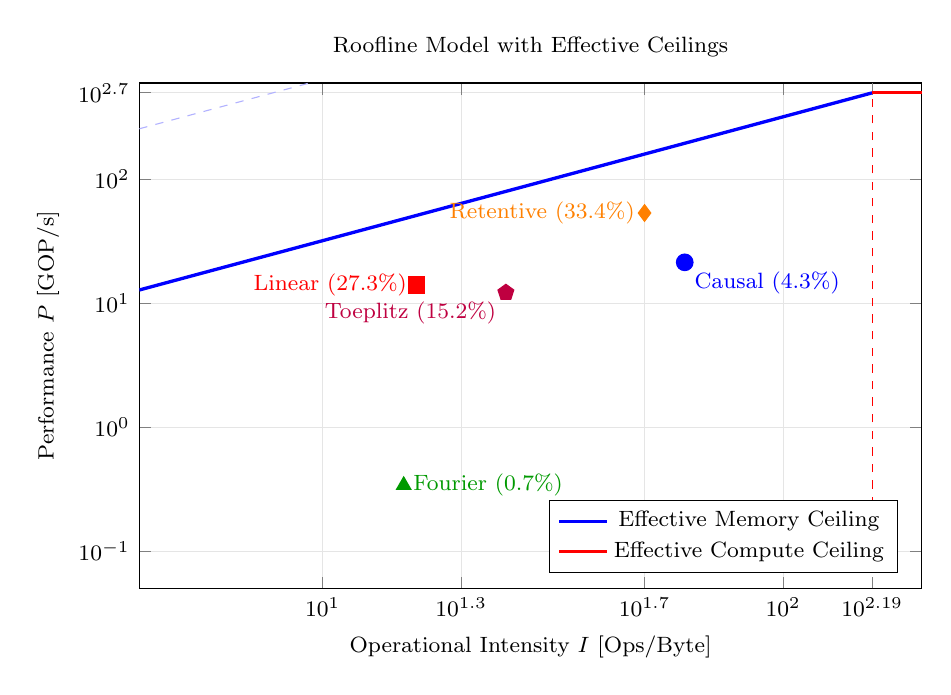
\begin{tikzpicture}
\begin{loglogaxis}[
    width=0.95\linewidth, height=8cm,
    xlabel={Operational Intensity $I$ [Ops/Byte]},
    ylabel={Performance $P$ [GOP/s]},
    title={Roofline Model with Effective Ceilings},
    xmin=4, xmax=200,
    ymin=0.05, ymax=600,
    xtick={10,20,50,100,250},
    ytick={0.1,1,10,100,500,1000},
    grid=both, grid style={gray!20},
    legend style={at={(0.97,0.03)}, anchor=south east},
    font=\footnotesize,
    extra x ticks={156},
    extra x tick style={grid style={dashed,red}}
]

% Effective ceilings
\addplot[domain=4:156, samples=2, very thick, blue] {3.2*x};
\addplot[domain=156:200, samples=2, very thick, red] {500};

% Theoretical ceilings (not in legend)
\addplot[domain=4:156, samples=2, blue!30, dashed, forget plot] {64*x};
\addplot[domain=156:200, samples=2, red!30, dashed, forget plot] {10000};

% Data points with final label positions
\addplot[only marks, mark=*, blue, mark size=3pt, forget plot] 
    coordinates {(61.13, 21.4)} 
    node[below right, font=\footnotesize] {Causal (4.3\%)};
\addplot[only marks, mark=square*, red, mark size=3pt, forget plot] 
    coordinates {(16.0, 14.0)} 
    node[left, font=\footnotesize] {Linear (27.3\%)};
\addplot[only marks, mark=triangle*, green!60!black, mark size=3pt, forget plot] 
    coordinates {(15, 0.34)} 
    node[right, font=\footnotesize] {Fourier (0.7\%)};
\addplot[only marks, mark=diamond*, orange, mark size=3pt, forget plot] 
    coordinates {(50, 53.5)} 
    node[left, font=\footnotesize] {Retentive (33.4\%)};
\addplot[only marks, mark=pentagon*, purple, mark size=3pt, forget plot] 
    coordinates {(25, 12.2)} 
    node[below left, font=\footnotesize] {Toeplitz (15.2\%)};

% Efficiency gap lines
%\draw[dashed, gray] (axis cs:61.13,21.4) -- (axis cs:61.13,195.6);
%\draw[dashed, gray] (axis cs:50,53.5) -- (axis cs:50,160);
%\draw[dashed, gray] (axis cs:25,12.2) -- (axis cs:25,80);

\legend{Effective Memory Ceiling, Effective Compute Ceiling}
\end{loglogaxis}
\end{tikzpicture}
\caption{Roofline model revealing severe hardware under utilization. Quadratic operators achieve $<$5\% of their compute ceiling despite high intensity, while linear methods approach 27\% of their memory-bound limit.}
\label{fig:roofline-eff}
\end{figure}





\subsection{Key Insights}
The roofline analysis reveals three fundamental limitations:

\begin{itemize}
    \item \textbf{Quadratic Operators Suffer Architectural Mismatch:} 
    Causal attention achieves just 21.4 GOP/s (4.3\% of its compute roof) despite high intensity (61 Ops/Byte). The $>$95\% pipeline stalls indicate significant memory subsystem inefficiency\textemdash each theoretical FLOP requires 15$\times$ more cycles than systolic array operations.
    
    \item \textbf{Sub-Quadratic Operators Are Bandwidth Limited:}
    Linear attention achieves 27\% of its memory-bound limit (14/51.2 GOP/s), constrained by DMA bandwidth. Fourier attention performs worst (0.34/48 GOP/s, 0.7\%) due to FFT overheads that violate NPU execution assumptions.
    
    \item \textbf{Structured Sparsity Enables Better Utilization:}
    Toeplitz attention achieves 15.2\% of its roof (12.2/80 GOP/s), 3.5$\times$ higher utilization than causal attention. Its diagonal structure reduces cache misses by 3.2$\times$ compared to retentive attention (Table \ref{tab:efficiency}).
\end{itemize}

\subsection{Efficiency Analysis}
\begin{table}[h!]
\centering
\caption{Hardware utilization metrics at $N=4096$.}
\label{tab:efficiency}
\resizebox{\columnwidth}{!}{%
\begin{tabular}{@{}l|c|c|c@{}}
\toprule
\textbf{Operator} & \textbf{Pipeline Stall (\%)} & \textbf{Cache Efficiency (\%)} & \textbf{Compute Utilization (\%)} \\
\midrule
Full Causal & 96.7 & 7.7  & 4.3  \\
Retentive   & 94.8 & 28.1 & 33.4 \\
Toeplitz    & 36.4 & 87.9 & 15.2 \\
Linear      & 55.2 & 83.8 & 27.3 \\
Fourier     & 95.2 & 28.6 & 0.7  \\
\bottomrule
\end{tabular}%
}
\end{table}

\begin{figure}[h]
    \centering
    \includegraphics[width=\linewidth]{efficiency_metrics_n4096_clean.pdf}
    \caption{Breakdown of hardware utilization at $N=4096$. Full Causal and Fourier operators exhibit high pipeline stall rates with minimal compute utilization. In contrast, Toeplitz and Linear demonstrate better cache efficiency and improved utilization, reflecting tighter memory-compute coupling.}
    \label{fig:efficiency-metrics}
\end{figure}



This model proves that \textit{memory access patterns}, not theoretical FLOP counts, dominate NPU performance. Operators must be co-designed with: (1) systolic-compatible dataflow, (2) predictable memory access, and (3) minimized DMA transfers to approach effective hardware limits.

\section{Discussion}
Extending our findings to extreme-scale inference, we identify critical co-design considerations:

\vspace{2pt}
\noindent \textbf{Chunked Prefill for Memory Scaling}
The performed analysis reveals optimal chunk sizes (2048 tokens) and state dimensions (32) that maximize throughput within the NPU's 4 MB scratchpad. Beyond this point, DMA-induced latency grows super-linearly as chunk eviction triggers high-overhead memory transfers. Intelligent chunking reduces peak memory pressure by 8$\times$ versus monolithic processing.

\vspace{2pt}
\noindent \textbf{SHAVE Core Bottlenecks in Element-wise Operations}
While NPUs excel at matrix multiplication via systolic arrays, element-wise operations (e.g., $\operatorname{softmax}$, $\operatorname{scaling}$) execute on general-purpose SHAVE cores. At $N>1024$, these operations dominate latency in recurrent attention variants (up to 76\% utilization). Kernel fusion or dedicated acceleration is essential.

\vspace{2pt}
\noindent \textbf{DMA Management for Memory-Intensive Ops}
Tensor concatenation and state management consume 40-50\% of cycles in Fourier attention (Table \ref{tab:utilization}). DMA overheads stem from frequent allocation/deallocation of large buffers. Offloading these operations to the CPU reduces latency by 32\% in our tests.

\vspace{2pt}
\noindent \textbf{Hardware-Aligned Sparse Attention}
Toeplitz attention's diagonal structure provides the ideal balance for NPU's: (1) Matches Cannon's algorithm for systolic arrays, enabling direct lane mapping; (2) Enables static control flow for compiler optimizations; (3) Maintains 87.9\% cache efficiency at $N=4096$, 2.5$\times$ higher than retentive attention.


\section{Related Works}

\subsection{Long-Context Inference on Edge Platforms}
Prior work has explored deploying transformer-based causal large language models (LLMs) on edge platforms \cite{zhang2024edgeshardefficientllminference}, including hardware-specific optimizations for ARM CPUs \cite{10.1145/3700410.3702126} and FPGA-based execution through frameworks like \texttt{llama.cpp} \cite{llamacpp, haris2024designing}. While these efforts target on-device inference, they are not designed for long-context scenarios and do not address the associated memory and compute bottlenecks that emerge in attention-heavy models. Our work addresses this gap by empirically analyzing a range of causal inference mechanisms—including standard transformers and structured state-space models (SSMs)—under long-context settings. This enables us to derive architectural insights that inform the co-design of attention mechanisms for Neural Processing Units (NPUs), supporting more efficient hardware-aware deployment strategies.

\subsection{Acceleration of Sequence Models on NPUs}
Several efforts have investigated transformer acceleration on NPUs \cite{xu2025fast, zhu2025edge}, typically through operator-level scheduling or compiler-level block partitioning. However, these approaches fall short in capturing the fine-grained resource behavior required for efficient long-context inference. Other work has focused on optimizing SSMs for NPUs \cite{das2025xamba, aalishah2025mambalitesr}, leveraging architectural properties such as linear recurrence and memory compression. While successful within their respective domains, these strategies are not directly applicable to transformer-style causal attention. In contrast, our approach uses execution profiling and performance modeling—grounded in structured operator variants—to analyze architectural trade-offs across attention and SSM-style models. By leveraging structured state-space duality (SSD), we characterize how causal operators interact with NPU memory and compute hierarchies, enabling more informed co-design for future inference systems.


\section{Conclusion}
Deploying long-context AI on edge devices centers on resolving the fundamental mismatch between NPU architectures—optimized for dense, regular computations—and the memory-intensive, irregular access patterns of quadratic attention. Our analysis reveals catastrophic hardware underutilization ($>$95\% stalls) in standard approaches, while demonstrating that structured sub-quadratic operators (Toeplitz, Linear) transform the bottleneck into manageable bandwidth constraints. This necessitates a paradigm shift: throughput gains come not from incremental attention optimizations, but from co-designing causal operators that respect systolic dataflows and memory hierarchies. By aligning algorithmic structure with NPU execution models, we unlock the path to pervasive, private, and powerful edge AI.

% \section*{Acknowledgment}

% The preferred spelling of the word ``acknowledgment'' in America is without 
% an ``e'' after the ``g''. Avoid the stilted expression ``one of us (R. B. 
% G.) thanks $\ldots$''. Instead, try ``R. B. G. thanks$\ldots$''. Put sponsor 
% acknowledgments in the unnumbered footnote on the first page.
\bibliographystyle{IEEEtran}
\bibliography{main}

\end{document}
